\section{GitHub}
\label{sec:git-github}

Already mentioned it a few times before (see p. \pageref{sec:jekyll}, \pageref{sec:buildpipelines-markdown} or \pageref{sec:git}), \emph{GitHub} is currently probably the most popular online collaboration platform, hosting not only the source code for the Linux kernel\footnote{\url{https://github.com/torvalds/linux} -- Linux kernel repository on GitHub.}, but also for other huge projects like Google's \emph{TensorFlow}\footnote{\url{https://github.com/tensorflow/tensorflow} -- Tensorflow repository on GitHub.}, Microsoft's \emph{.NET}\footnote{\url{https://github.com/Microsoft/dotnet} -- .NET repository on GitHub.} or Facebook's \emph{React}\footnote{\url{https://github.com/facebook/react} -- React repository on GitHub.}.

\subsection{History}
\label{sec:github-history}
Tom Preston-Werner, a Ruby programmer from San Francisco and creator of earlier mentioned Jekyll (see ch. \ref{sec:jekyll} on p. \pageref{sec:jekyll}) and \emph{Chris Wanstrath} started developing GitHub in October 2007. After releasing a private beta in January, they released the site to the public on April 10\textsuperscript{th}, 2008 \cite{PrestonWerner2008githublaunch}.

Since then, GitHub grew very fast and quickly gained on popularity throughout the developer landscape, hosting more than 56 million projects today\footnote{\url{https://github.com/about} -- GitHub's ``about'' page.}. Thanks to their generous freemium pricing model, collaborating in open source projects still is for free: A free tier account may hold unlimited open source repositories, working together with unlimited contributors\footnote{\url{https://github.com/pricing} -- GitHub's pricing page.}. All in all it seems, that GitHub turned coding into a truly social activity \cite[416]{loeliger2012version}.

\subsection{Technology}
The main use case for creating a repository on GitHub is the fact, that unlike other privately hosted remote repositories, it offers a wide range of additional services. Services like \emph{Issue tracking, Pull requests} and \emph{Code reviews} leverage the maintainability of source code in a repository, making it easy for each developer to discuss and manage the current project state without the need of switching to a third party application.

%% Screenshot of GitHub in-page editor
\begin{figure} % h-ere, t-op, b-ottom, p-age
    \centering
    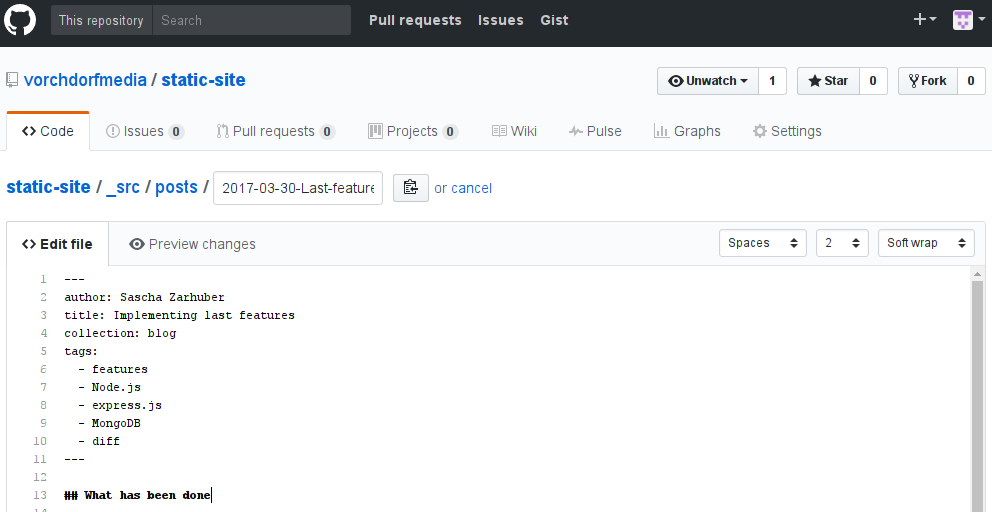
\includegraphics[width=0.9\textwidth]{github-page-editor.png}
    \caption{A Screenshot showing the \emph{In-Page Code Editor} of GitHub. An existing file is selected and ready to be edited. When finished, the user may commit the changes into the repository, so that other contributors also benefit from his/her adjustments.}
    \label{fig:github-page-editor}
\end{figure}
%

Especially for content authors without programming knowledge, the \emph{In-Page Code Editor} might be a very supportive tool, as it provides a clean and easy-to-use frontend for directly adding content to the repository (see Fig. \ref{fig:github-page-editor}). Additionally, the just edited file may not only be committed into the currently selected branch, but also in a newly created branch. Therefore, the source branch stays clean, whereas the edited file may get reviewed by an assigned supervisor, before being ready to get merged.\\
Furthermore, also developers might make use of this feature, especially when a small hotfix is to be made, where it would be too time-consuming to \emph{pull, commit} and \emph{push} from/to the repository \cite[405]{loeliger2012version}.

Pushing to a \emph{gh-pages} branch, or creating a \emph{<username>.github.io} repository, enables the use of GitHub's built-in website hosting service. From there, either a Jekyll project is freshly built, or already compiled static HTML are automatically published to the web -- additionally, custom domains may be used when adding a \texttt{CNAME} file \cite[p. 171f]{dhillon2016}.

\subsection{REST API}
Another significant advantage is the access of GitHub's REST API. Currently existing in its third major release, it almost offers every feature also available graphically in its web interface, as an equivalent JavaScript Object Notation (\emph{JSON}) upon programmatical request. Some services even feature more advanced data through the API than through the UI \cite[410]{loeliger2012version}.

When having the need of including data from a GitHub account into a third party service, a single authenticated HTTP request does the trick. Due to many available endpoints, a developer may quickly find the type information he/she needs to further process data directly from a repository. As an example, a complete listing of a repository's file tree is also possible, without needing to download and unpack an archive file. For one thing, this saves quite some time, for another thing, the requested data is already processed and presented, so that not only file paths are unveiled, but also their direct links and data types.

Furthermore, the API not only offers access to informational data about a given repository, instead, its manipulation through creating commits or uploading a file may also happen. To sum this up, very well documented examples are available on the API page on GitHub, where developers catch a good glimpse, of what is possible overall\footnote{\url{https://developer.github.com/v3/} -- API v3 documentation on GitHub.} \cite[401]{loeliger2012version}.
